\documentclass[varwidth=10in]{standalone}
\usepackage{tikz-qtree}

\begin{document}

{\Huge 5}
\qquad
{\Huge + }
\qquad
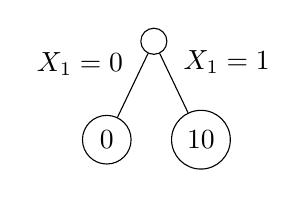
\begin{tikzpicture}[every tree node/.style={draw,circle},
   level distance=1.25cm,sibling distance=.5cm, 
   edge from parent path={(\tikzparentnode) -- (\tikzchildnode)}]

\Tree
    [.\node {};
      \edge node[auto=right] {$X_1 = 0$};  
      [.0  ] 
      \edge node[auto=left] {$X_1 = 1$};  
 [.10 ]
    ]
  

\end{tikzpicture}
\qquad
{\Huge +}
\qquad
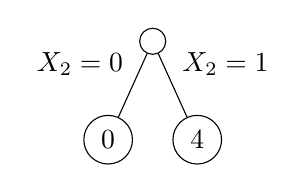
\begin{tikzpicture}[every tree node/.style={draw,circle},
   level distance=1.25cm,sibling distance=.5cm, 
   edge from parent path={(\tikzparentnode) -- (\tikzchildnode)}]

\Tree [.\node {}; 
      \edge node[auto=right] {$X_2 = 0$};  
    [.0  ] 
      \edge node[auto=left] {$X_2 = 1$};  
[.4 ]
]

\end{tikzpicture}


\end{document}